\documentclass[12pt, a4paper, oneside]{ctexart}
\usepackage{amsmath, amsthm, amssymb, appendix, bm, graphicx, hyperref, mathrsfs,adjustbox}
\usepackage{enumerate}
\title{\textbf{论文标题}}
\author{tanghongyu}
\date{\today}
\linespread{1.5}
\newtheorem{theorem}{定理}[section]
\newtheorem{definition}[theorem]{定义}
\newtheorem{lemma}[theorem]{引理}
\newtheorem{corollary}[theorem]{推论}
\newtheorem{example}[theorem]{例}
\newtheorem{proposition}[theorem]{命题}
\renewcommand{\abstractname}{\Large\textbf{摘要}}

\begin{document}

\maketitle

\setcounter{page}{0}
\maketitle
\thispagestyle{empty}

\begin{abstract}
    这里是摘要.
    \par\textbf{关键词:}这里是关键词; 这里是关键词.
\end{abstract}

\newpage
\pagenumbering{Roman}
\setcounter{page}{1}
\tableofcontents
\newpage
\setcounter{page}{1}
\pagenumbering{arabic}

\section{一级标题}

\subsection{二级标题}

\begin{theorem}

\end{theorem}

\begin{table}[htbp]
    \centering  % 显示位置为中间
    \caption{ }  % 表格标题
    \label{tab2}  % 用于索引表格的标签
    %字母的个数对应列数,|代表分割线
    % l代表左对齐,c代表居中,r代表右对齐
    \begin{adjustbox}{max width=\textwidth}
        \begin{tabular}{|c|c|c|}
            \hline
            $ $          & 原始Paillier算法                                                  & 改进后Paillier算法                                                                 \\
            \hline
            $KeyGen$     & $ n = pq ,$                                                   & $ n = PQ,P=2pp'+1, Q=2qq'+1$                                                  \\
            \hline
            $Encryption$ & $c = g^{m}r^{n} \bmod n^2,r \stackrel{R}{\leftarrow} {Z_n^*}$ & $ c = (1+mn)(-y^{2p'q'})^{nr} \bmod n^2,r \stackrel{R}{\leftarrow} \{0,1\}^l$ \\
            \hline
            $Decryption$ & $m = L_n(c^{\lambda }\bmod n^2)\cdot \mu \bmod n$             & $m = L_n(c^{2pq} \bmod n^2)\cdot (2pq)^{-1} \bmod n $                         \\
            \hline
        \end{tabular}
    \end{adjustbox}
\end{table}

$g^{\alpha n} = 1 mod n^2,\alpha \in \{ 1,2,\cdots,\lambda\}$即$g = (1+n)^x\cdot y^n mod n^2$(一般取$1+n$),对于$ \lambda = lcm(p-1,q-1),\mu = L(g^{\lambda} \bmod n^2)^{-1} \bmod n^2$,
又$r^{\lambda\cdot n}=1\bmod n^2$,则$c^{\lambda }\bmod n^2 = (1+n)^{xm}\bmod n^2 = (1+xmn)\bmod n^2$。同理$\mu = L((1+xn)\bmod n^2)^{-1}\bmod n$,
故可以成功解密。$(1+n)^m = (1+mn) \bmod n^2$可以减少模指数运算。
\par

对于$y\in Z_{n}^*$,$(-y^2)^{p'q'} \bmod n\in QR_n^{n-l}$。随机取$r\in\{ 0,1\}^l$,则$(-y^2)^{rp'q'} \bmod n$在计算上为$Z^*_n\left [ +1\right ]$上的随机元素。
其中指数为$r$,从而可以提升效率。
\par
\begin{equation}
    \begin{split}
        c&=\\
        &=(h^r\bmod n)^n \bmod n^2\\
        &=(h^r+x\cdot n) ^n \bmod n^2,x\in \{-n+1,\cdots,n-1\}\\
        &=h^{rn}+ xnh^{r(n-1)}\bmod n^2
    \end{split}
\end{equation}

又$n|h^{r(n-1)}$,故$n^2|xnh^{r(n-1)}$\par

由$\phi(P^2) = P(1-P) = 2pp'P $,$(-y^{2p'q'})^{2pnr} = 1\bmod P^2$,

\begin{equation}
    \begin{split}
        c_p &= (1+mn)^{2p} \bmod P^2\\
        &=1+2pmn \bmod P^2\\
        &=1+2pPQm \bmod P^2
    \end{split}
\end{equation}

$c_p = m \bmod P^2,c_q = m \bmod Q^2$,由CRT,$m = c_pQ(Q^{-1}\bmod P)+ c_qP(P^{-1}\bmod Q) \bmod N$。
又$Q(Q^{-1}\bmod P) + P(P^{-1}\bmod Q) = 1\bmod n$,故$m=c_p+h_q\cdot P\cdot (P^{-1}  \bmod Q)  \bmod N$。
\par

$\alpha =\alpha_1 +\alpha_2 = m_1+m_2-b_1-b_2$,
$\beta = \beta_1 \cdot \beta_2 = Enc_{pk}(b_1+b_2)$,
故可以成功解密。
\par

密文$(\alpha_{11},\beta_{11}),(\alpha_{12},\beta_{12}),(\alpha_{21},\beta_{21}),(\alpha_{22},\beta_{22})$,
进行第一轮乘法同态加密,得到
$$ \alpha_1 = Enc_{pk}(\alpha_{11}\cdot \alpha_{12}) (\beta_{11})^{\alpha_{12}}(\beta_{12})^{\alpha_{11}}$$
$$ \alpha_2 = Enc_{pk}(\alpha_{21}\cdot \alpha_{22}) (\beta_{21})^{\alpha_{22}}(\beta_{22})^{\alpha_{21}}$$
进行第二轮加法同态加密,得到
$$ \alpha=\alpha_1\cdot \alpha_2,\beta_1 = \beta_{11}\cdot \beta_{12},\beta_2 = \beta_{21}\cdot \beta_{22}$$
解密得到

\begin{equation}
    \begin{split}
        Dec_{sk}(\alpha) &= \alpha_{11}\cdot \alpha_{12} + \alpha_{12}\cdot b_{11}+ \alpha_{11}\cdot b_{12}
        + \alpha_{21}\cdot \alpha_{22} + \alpha_{22}\cdot b_{21}+ \alpha_{21}\cdot b_{22}\\
        &=(m_{11}-b_{11})(m_{12}-b_{12})+(m_{12}-b_{12})b_{11}+(m_{11}-b_{11})b_{12}\\
        &+(m_{21}-b_{21})(m_{22}-b_{22})+(m_{22}-b_{22})b_{21}+(m_{21}-b_{21})b_{22}\\
        &= m_{11}\cdot m_{12}-b_{11}b_{12}+m_{21}\cdot m_{22}-b_{21}b_{22}
    \end{split}
\end{equation}

$$(Dec_{sk}(\beta_1)Dec_{sk}(\beta_2)) = (b_{11}+b_{12})(b_{21}+b_{22}) $$

\newpage

\begin{table}[htbp]
    \centering  % 显示位置为中间
    \caption{ }  % 表格标题
    \label{tab1}  % 用于索引表格的标签
    %字母的个数对应列数,|代表分割线
    % l代表左对齐,c代表居中,r代表右对齐
    \begin{tabular}{|c|c|c|}
        \hline
        $ 运行时间$      & 原始Paillier算法 & 改进后Paillier算法 \\
        \hline
        $KeyGen$     & 1.36039 s    & 2.19955 s     \\
        \hline
        $Encryption$ & 0.145491 s   & 0.0217804 s   \\
        \hline
        $Decryption$ & 0.0490871 s  & 0.0107389 s   \\
        \hline
    \end{tabular}
\end{table}


\begin{table}[htbp]
    \centering  % 显示位置为中间
    \caption{ }  % 表格标题
    \label{tab111}  % 用于索引表格的标签
    %字母的个数对应列数,|代表分割线
    % l代表左对齐,c代表居中,r代表右对齐
    \begin{tabular}{|c|c|}
        \hline
        加密4k字节数据的运行效率 & SM4-ECB    \\
        \hline
        改进后$AVX-512$  & 30341 Mb/s \\
        \hline
        改进后$AVX-256$  & 5030 Mb/s  \\
        \hline
        $AVX-256$     & 2300 Mb/s  \\
        \hline
        原始版           & 732 Mb/s   \\
        \hline
    \end{tabular}
\end{table}


\begin{table}[htbp]
    \centering  % 显示位置为中间
    \caption{ }  % 表格标题
    \label{tab333}  % 用于索引表格的标签
    %字母的个数对应列数,|代表分割线
    % l代表左对齐,c代表居中,r代表右对齐
    \begin{tabular}{|c|c|}
        \hline
        加密128字节数据的运行效率 & SM4-GCM  \\
        \hline
        改进后$AVX-512$   & 400 Mb/s \\
        \hline
        改进后$AVX-256$   & 326 Mb/s \\
        \hline
        $AVX-256$      & 258 Mb/s \\
        \hline
        原始版            & 253 Mb/s \\
        \hline
    \end{tabular}
\end{table}

\begin{table}[htbp]
    \centering  % 显示位置为中间
    \caption{ }  % 表格标题
    \label{tab222}  % 用于索引表格的标签
    %字母的个数对应列数,|代表分割线
    % l代表左对齐,c代表居中,r代表右对齐
    \begin{tabular}{|c|c|}
        \hline
        加密128字节数据的运行效率 & SM4-GCM   \\
        \hline
        改进后$AVX-512$   & 2528 Mb/s \\
        \hline
        改进后$AVX-256$   & 918 Mb/s  \\
        \hline
        $AVX-256$      & 1374 Mb/s \\
        \hline
        原始版            & 513 Mb/s  \\
        \hline
    \end{tabular}
\end{table}

\newpage


\section{同态加密方案}
符号说明:明文$m\in M$,密文$c\in C$,并且$Enc_{pk} (m),Dec_{sk} (c)$表示使用公钥$pk$或私钥$sk$的原始Paillier加密算法进行加解密。$\oplus$表示密文的同态加法,$\odot$表示为密文的同态乘法。

同态加密密文初始化为$C\in M \times C$,其中$C=\left (a,\beta\right )$。取随机数$b\in M$,分别计算$a=m-b,\beta=Enc_{pk}\left (b\right )$。

\subsection{一级同态加密加法和常量乘法}
对于Level = 1的密文同态加法计算,对于输入密文$C_i=\left (a_i,\beta_i\right ),i=1,2$,通过以下计算可得到密文 $C_{add1}\in M\times C$。
$$C_{add1}=C_1\oplus C_2=(a_1+a_2,\beta_1\cdot\beta_2)$$
\par
对于Level = 1的密文同态标量乘法计算,对于任意$k\in Z$,对于输入密文$C=\left (a,\beta\right )$,通过以下计算可得到密文$C_{cm1}\in M\times C$。
$$C_{cm1}=k\cdot C=\left (ka,\beta ^k\right )$$
\par
对于level-1的密文$C=\left (a,\beta\right )$,利用私钥$sk$对密文解密:$Dec\left (C\right )=a+Dec_{sk}\left (\beta\right )$。对于$C_{add1}=C_1\oplus C_2$与$C_{cm1}=k\cdot C$解密正确性为
$$Dec\left (C_{add1}\right )=a_1+a_2+Dec_{sk}\left (\beta_1\cdot\beta_2\right )=a_1+a_2+b_1+b_2=m_1+m_2$$
$$Dec\left (C_{cm1}\right )=ka+Dec_{sk}\left (\beta^k\right )=ka+kb=km$$

\subsection{一级同态乘法加密与二级同态加密加法和常量乘法}
对于Level = 1的密文同态乘法计算,对于输入密文$C_i=\left (a_i,\beta_i\right ),i=1,2$,
通过以下计算可得到密文$C_{mul1}\in C^3$。
$$C_{mul1}=C_1\odot C_2 = (\alpha ,\beta_1,\beta_2)$$
其中:$\alpha = Enc_{pk}(\alpha_1\cdot \alpha_2)\cdot \beta_1^{\alpha_2}\cdot \beta_2^{\alpha_1}$。

对于Level = 2的密文同态加法计算,对于输入密文$C_i=\left (a_i,\beta_{1,i},\beta_{2,i}\right ),i=1,2$,
通过以下计算可得到密文$C_{add2}\in C^3$。
$$C_{add2} =  C_1\oplus C_2=(\alpha_1\cdot \alpha_2,(\beta_{1,1},\beta_{1,2}),(\beta_{2,1},\beta_{2,2}))$$

对于Level = 2的密文同态标量乘法计算,对于任意$k\in Z$,对于输入密文$C=\left (\alpha,\beta_1,\beta_2\right )$,
通过以下计算可得到密文$C_{cm2}\in M\times C$。
$$C_{cm1}=k\cdot C=\left (\alpha^k,(\beta_{1},\cdots,\beta_{1}),(\beta_{2},\cdots,\beta_{2})\right )$$

对于Level = 2的密文$C=\left (\alpha,\beta_1,\beta_2\right )$,并且$\beta_1,\beta_2$为两个$k$元组,
利用私钥$sk$对密文解密:$Dec(C) = Dec_{sk}(\alpha)+ \sum_{i=1}^{k}(Dec_{sk}(\beta_1[i])\cdot Dec_{sk}(\beta_2[i]))$。

该解密方法对于Level = 1的密文同态乘法计算的正确性为,
\begin{equation}\label{alpha}
    \begin{split}
        Dec_{sk}(\alpha) &= (a_1\cdot a_2)+(a_2\cdot b_1)+(a_1\cdot b_2)\\
        &= m_1m_2-m_1b_2-m_2b_1+b_1b_2+m_2b_1-b_1b_2+m_1b_2-b_1b_2\\
        &= m_1m_2-b_1b_2
    \end{split}
\end{equation}
又$ Dec_{sk}(\beta_1)\cdot Dec_{sk}(\beta_2) = b_1b_2$,
故$m_1m_2 = Dec_{sk}(\alpha) +Dec_{sk}(\beta_1)\cdot Dec_{sk}(\beta_2)$。

对于Level = 2的密文同态加法计算,若$C_1,C_2$分别由明文$m_1,m_2,m_3,m_4$
所生成的密文通过两次Level = 1的密文同态乘法计算得到,
则由\ref{alpha}可知
\begin{equation}
    \begin{split}
        Dec_{sk}(\alpha_1\cdot \alpha_2)&= Dec_{sk}(\alpha_1)+Dec_{sk}(\alpha_2)\\
        &= m_1m_2-b_1b_2+m_3m_4-b_3b_4
    \end{split}
\end{equation}
且$Dec_{sk}(\beta_{1,1})\cdot Dec_{sk}(\beta_{2,1}) = b_1b_2$,$Dec_{sk}(\beta_{1,2})\cdot Dec_{sk}(\beta_{2,2}) = b_3b_4$,
故通过上述过程可解密得到$m_1m_2+m_3m_4$,Level = 2的密文同态标量乘法计算同理。

\subsection{二级同态加密乘法}
若对明文$m_1,m_2,m_3,m_4$进行初始化,得到密文$C_i=(a_i,\beta_i),i=1,2,3,4$。
对于二级同态加密乘法,我们考虑两种情况,
\begin{enumerate}[(1)]
    \item $C_1,C_2$通过Level = 1的密文同态乘法计算得到$C_{mul1}=C_1\odot C_2 $,而后计算$C_{mul2}=C_{mul1}\odot C_3 $;
    \item $C_1,C_2$与$C_3,C_4$通过Level = 1的密文同态乘法计算分别得到$C_{mul1}=C_1\odot C_2 $与$C'_{mul1}=C_3\odot C_4 $,而后计算$C_{mul2}=C_{mul1}\odot C'_{mul1} $。
\end{enumerate}

令$C_{mul2}$为一个四元组$ (\Delta_1,\Delta_2,\Delta_3,(\beta_1,\cdots,\beta_n))$,
并且记$C_{mul1}= (\alpha,\beta_1,\beta_2),C'_{mul1}= (\alpha',\beta_3,\beta_4)$。

在情况1下,$C_{mul2}=C_{mul1}\odot C_3 = (\alpha^{a_3},(\beta_1^{a_3},\beta_2),(\alpha,\beta_3),(\beta_1,\beta_2,\beta_3))$;
在情况2下,$C'_{mul2}=C_{mul1}\odot C'_{mul1} =((\alpha,\alpha'),(\alpha',\beta_1,\beta_2),(\alpha, \beta_3,\beta_4),(\beta_1,\beta_2,\beta_3,\beta_4))$。

二级同态加密乘法的解密算法为

$Dec(C_{mul2}) = Dec(\Delta_1)+Dec(\Delta_2)+Dec(\Delta_3)+\prod_{i=1}^n(Dec(\beta_i))$。

对于情况1,$Dec(\Delta_1) = Dec_{sk}(\alpha^{a_3}) $,由\ref{alpha}可知,
$Dec(\Delta_1) = (m_3-b_3)(m_1m_2-b_1b_2)=m_1m_2m_3-m_1m_2b_3-m_3b_1b_2+b_1b_2b_3$,

$Dec(\Delta_2) = Dec_{sk}((\beta_1)^{a_3})Dec_{sk}(\beta_2) =m_3b_1b_2-b_1b_2b_3 $,

$Dec(\Delta_3) = Dec_{sk}(\beta_3)Dec_{sk}(\alpha) =m_1m_2b_3-b_1b_2b_3 $,则$Dec(C_{mul2}) = m_1m_2m_3$。

对于情况2,$Dec(\Delta_1) = Dec_{sk}(\alpha)Dec_{sk}(\alpha') $,由\ref{alpha}可知,

$Dec(\Delta_1) = (m_1m_2-b_1b_2)(m_3m_4-b_3b_4)=m_1m_2m_3m_4-m_1m_2b_3b_4-m_3m_4b_1b_2+b_1b_2b_3b_4$,

$Dec(\Delta_2) = Dec_{sk}(\alpha')Dec_{sk}(\beta_1)Dec_{sk}(\beta_2) =m_3m_4b_1b_2-b_1b_2b_3b_4 $,

$Dec(\Delta_3) = Dec_{sk}(\alpha)Dec_{sk}(\beta_3)Dec_{sk}(\beta_4) =m_1m_2b_3b_4-b_1b_2b_3b_4 $,
则$Dec(C'_{mul2}) = m_1m_2m_3m_4$。

\subsection{三级同态加密加法和模乘}

设有8个明文$m_{1,1},m_{1,2},m_{1,3},m_{1,4},m_{2,1},m_{2,2},m_{2,3},m_{2,4}$,
分别初始化密文为$C_{1,1},C_{1,2},C_{1,3},C_{1,4},C_{2,1},C_{2,2},C_{2,3},C_{2,4}$。

两两进行一级同态加密乘法,即$C_{mul1,1} = C_{1,1}\odot C_{1,2},C_{mul1,2} = C_{1,3}\odot C_{1,4}$,
$C_{mul1,3} = C_{2,1}\odot C_{2,2},C_{mul1,4} = C_{2,3}\odot C_{2,4}$。

对密文$C_{mul1,1},C_{mul1,2},C_{mul1,3},C_{mul1,4}$两两进行二级同态加密乘法得
$C_{mul2,2} = C_{mul1,1}\odot C_{mul1,2},C'_{mul2,2} = C_{mul1,3}\odot C_{mul1,4}$为二级同态加密乘法的第二种情况。
其中$C_{mul2,2} = (\Delta_{1,2},\Delta_{2,2},\Delta_{3,2},( \{\beta_{1,i}|i=1,2,3,4\}))$
$$ = ((\alpha_1,\alpha_2),(\alpha_2,\beta_{1,1},\beta_{1,2}),(\alpha_1,\beta_{1,3},\beta_{1,4}) ,(\{\beta_{1,i}|i=1,2,3,4\})).$$
$C'_{mul2,2} = (\Delta'_{1,2},\Delta'_{2,2},\Delta'_{3,2},(\{\beta_{2,i}|i=1,2,3,4\}))$同理。

对密文$C_{mul1,1},C_{1,3},C_{mul1,2},C_{1,4}$进行二级同态加密乘法得
$C_{mul2,1} = C_{mul1,1}\odot C_{1,3},C'_{mul2,1} = C_{mul1,3}\odot C_{2,3}$为二级同态加密乘法的第一种情况。
其中$C_{mul2,1} = (\Delta_{1,1},\Delta_{2,1},\Delta_{3,1},(\{\beta_{1,i}|i=1,2,3\}))$
$$ =(\alpha_1^{a_{1,3}},(\beta_{1,1}^{a_{1,3}},\beta_{1,2}),(\alpha_1,\beta_{1,3}) ,(\{\beta_{1,i}|i=1,2,3\})) .$$
$C'_{mul2,1} = (\Delta'_{1,1},\Delta'_{2,1},\Delta'_{3,1},(\{\beta_{2,i}|i=1,2,3\}))$同理。

三级同态加密加法分为三种情况:
\begin{enumerate}[(1)]
    \item $C_{add3,1} = C_{mul2,1}\oplus C'_{mul2,1}$;
    \item $C_{add3,2} = C_{mul2,1}\oplus C_{mul2,2}$;
    \item $C_{add3,3} = C_{mul2,2}\oplus C'_{mul2,2}$。
\end{enumerate}
\begin{equation}
    \begin{split}
        C_{add3,1} =& (\alpha_1^{a_{1,3}}\alpha_3^{a_{2,3}},(\beta_{1,1}^{a_{1,3}},\beta_{1,2},\beta_{2,1}^{a_{2,3}},\beta_{2,2}),\\
        &(\alpha_1\alpha_3,\beta_{1,3},\beta_{2,3}),(\{\beta_{j,i}|i=1,2,3,j=1,2\}))
    \end{split}
\end{equation}


\begin{equation}
    \begin{split}
        C_{add3,2} =& (\alpha_1^{a_{1,3}}\alpha_3^{a_{2,3}},(\beta_{1,1}^{a_{1,3}},\beta_{1,2},\beta_{2,1}^{a_{2,3}},\beta_{2,2}),\\
        &(\alpha_1\alpha_3,\beta_{1,3},\beta_{2,3}),(\{\beta_{j,i}|i=1,2,3,j=1,2\}))
    \end{split}
\end{equation}

\newpage

$U = ABR^2 \bmod M M^{-1}\bmod R $\\

$C = \frac{ABR^2+ABR^2\cdot M}{R}$\\

\begin{figure*} [htbp!]
    \centering
    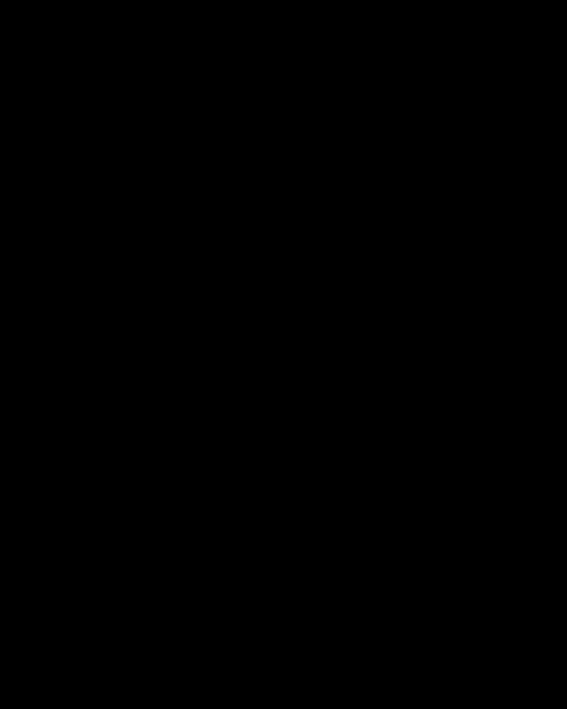
\includegraphics[scale=0.5]{fig.png}
    \caption{图1}
    \label{fig1}
\end{figure*}
\begin{thebibliography}{99}
    \bibitem{a}作者. \emph{文献}[M]. 地点:出版社,年份.
    \bibitem{b}作者. \emph{文献}[M]. 地点:出版社,年份.
\end{thebibliography}

\begin{appendices}
    \renewcommand{\thesection}{\Alph{section}}
    \section{附录标题}
    这里是附录.
\end{appendices}

\end{document}